\documentclass{article}
\usepackage{style}
\begin{document}
\maketitle
\part{Introducción}
\section{Neural Networks}

\subsection{Usos principales de las redes neuronales}

Se tienen 4 usos principales de las redes neuronales artificiales (RNA)
\begin{enumerate}
	\item Aproximación de sistemas (Modo regresor)
	\item Predicción de series de tiempo (Modo regresor)
	\item Control de Sistemas (Modo regresor)
	\item Clasificación de objetos (Modo Clasificador)
\end{enumerate}
\subsection{Aproximación de Sistemas}
Dado un sistema $f(t_i)$ del cuál se desconoce su modelo matemático, pero se cuenta con un conjunto de datos entrada-salida $(p, t)$ que representa su comportamiento. Se puede entrenar una RNA para que se comporte de manera similar a $f(t_i)$ en donde:\\\\
$t_i$ : Es la variable de tiempo\\
$p$ : Es la entrada (input)\\
$t$ : El valor deseado (target)\\

\subsection{Modelo Matemático}
Es una representación abstracta que aproxima al comportamiento de un fenómeno real, normalmente mediante un conjunto de ecuaciones.

\subsection{Ecuación}
Igualdad

\subsection{Datos input-output}
Es un conjunto de valores que muestrea mediante sensores el comportamiento dinámico del sistema en todo su rango de funcionamiento

\subsection{Buena Interpolación}
Se llama generación de conocimiento

\subsection{Mala Interpolación}
Se le llama sobrentendimiento

\textbf{LA RED EN MODO REGRESIÓN FUNCIONA COMO UN INTERPOLADOR}

\subsection{Extrapolar}
Pronosticar o predecir, se requieren RNA's recurrentes.

\subsection{Diagrama General}
\begin{figure}[h]
	\caption{Diagrama General}
	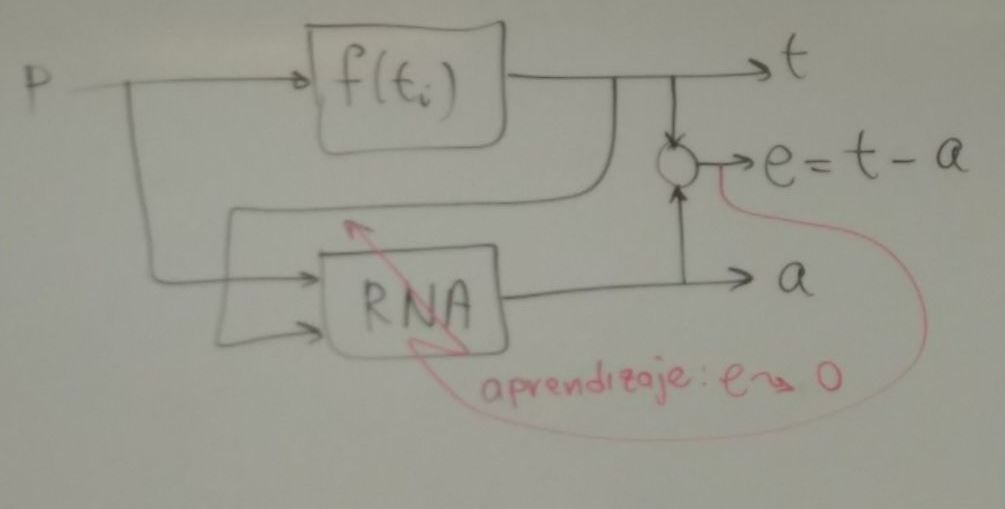
\includegraphics[scale=0.6]{modeloGeneralRn}
\end{figure}

\section{Tipos de Aprendizaje}
\subsection{Aprendizaje Supervisado}
Es aquel en el que se cuenta con ejemplos que contienen valores deseados(target) para llevar a cabo el ajuste de los parámetros de la RNA. En este caso se cuenta con un conjunto de datos$(p, t)$;

\subsection{Aprendizaje no Supervisado}
No se cuenta con ejemplos que contengan valores deseados. Sin embargo, existen diversos algoritmos en esta clasificación que se usan para analizar y extraer información valiosa de una fenómeno, por ejemplo, el algoritmo $k-medias$ recibe como entrada un conjunto de datos y un valor $k$ que representa el número de clases en los que se desea separar a dicho conjunto. Dependiendo del valor de $k$ el usuario podrá analizar de diferentes maneras el fenómeno.

\section{Predicción de Series de tiempo}
Dada una serie de tiempo que representa un fenómeno físico, existe un tiempo especial de RNA que es capaz de pronosticar valores futuros, es decir, realiza la correcta extrapolación de datos. Para esta tarea se hace uso de las RNA's recurrrentes.
\begin{figure}
	\centering
	\caption{Ejemplo de extrapolación}
	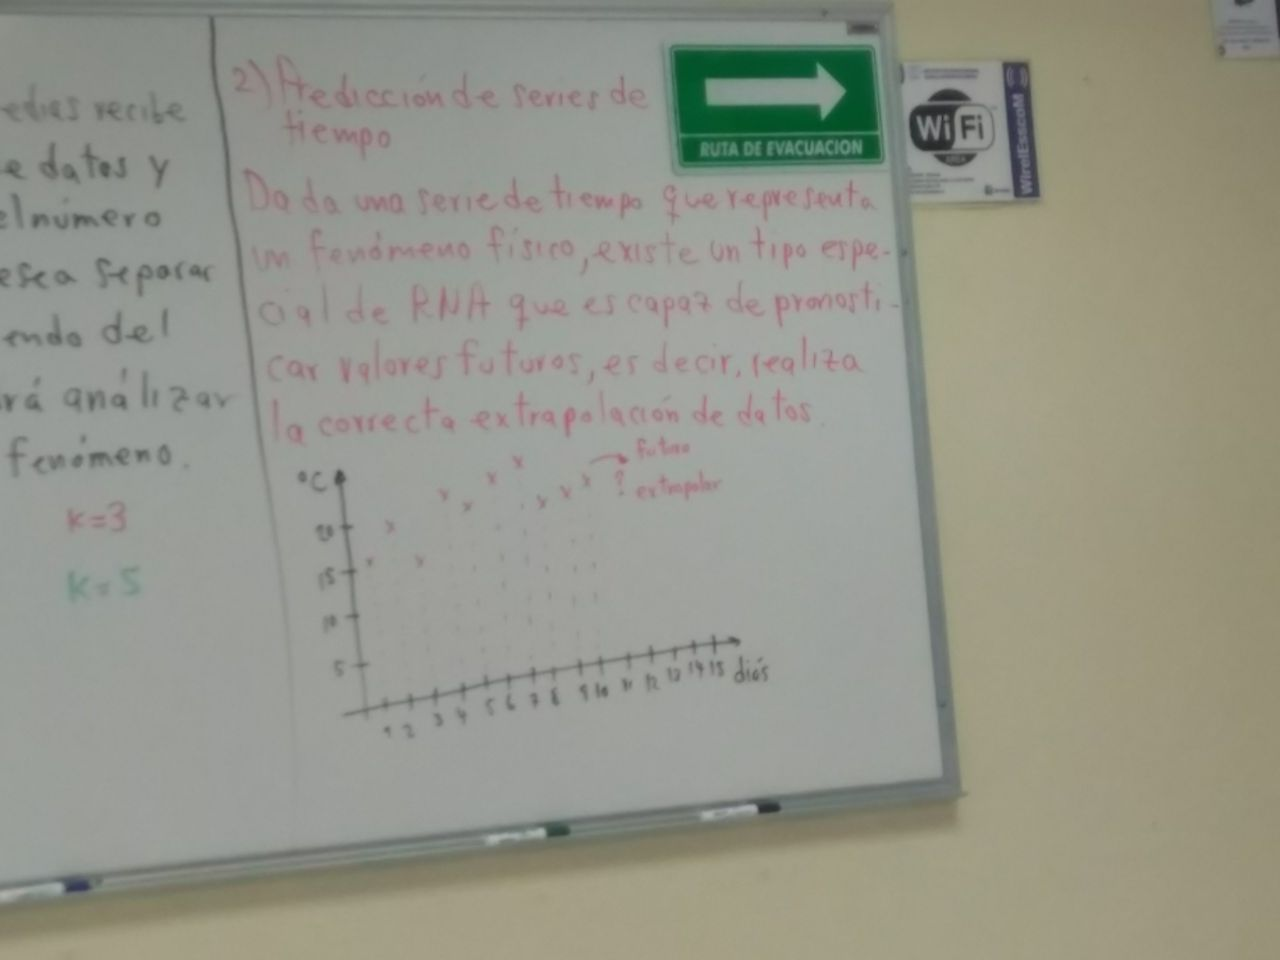
\includegraphics[scale=.4]{exampleTime}	
\end{figure}

\begin{figure}
	\centering
	\caption{Red Feed Foward}
	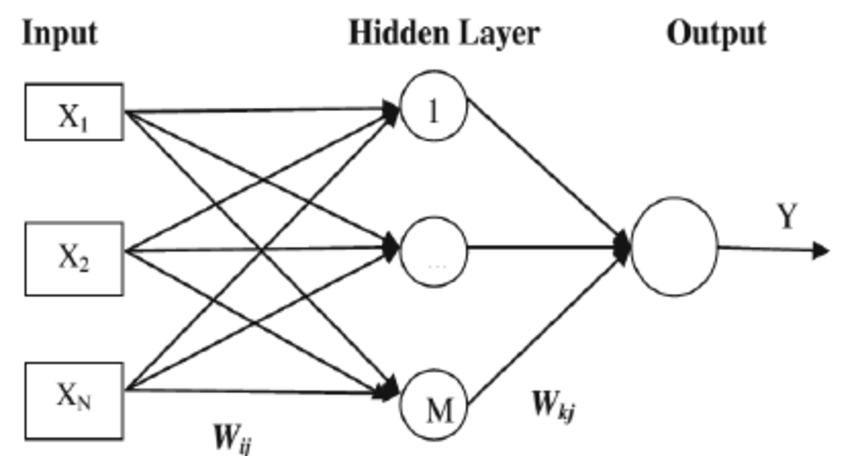
\includegraphics[scale=.5]{feedFowardExample}	
\end{figure}

\begin{figure}
	\centering
	\caption{Red Recurrente}
	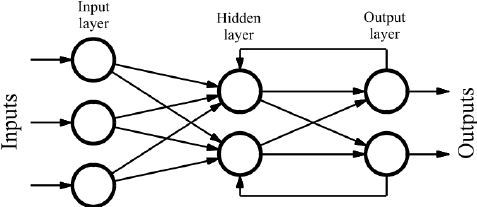
\includegraphics[scale=.8]{recurrentExample}	
\end{figure}

\begin{figure}
	\centering
	\caption{Red Recurrente con bloques recurrentes}
	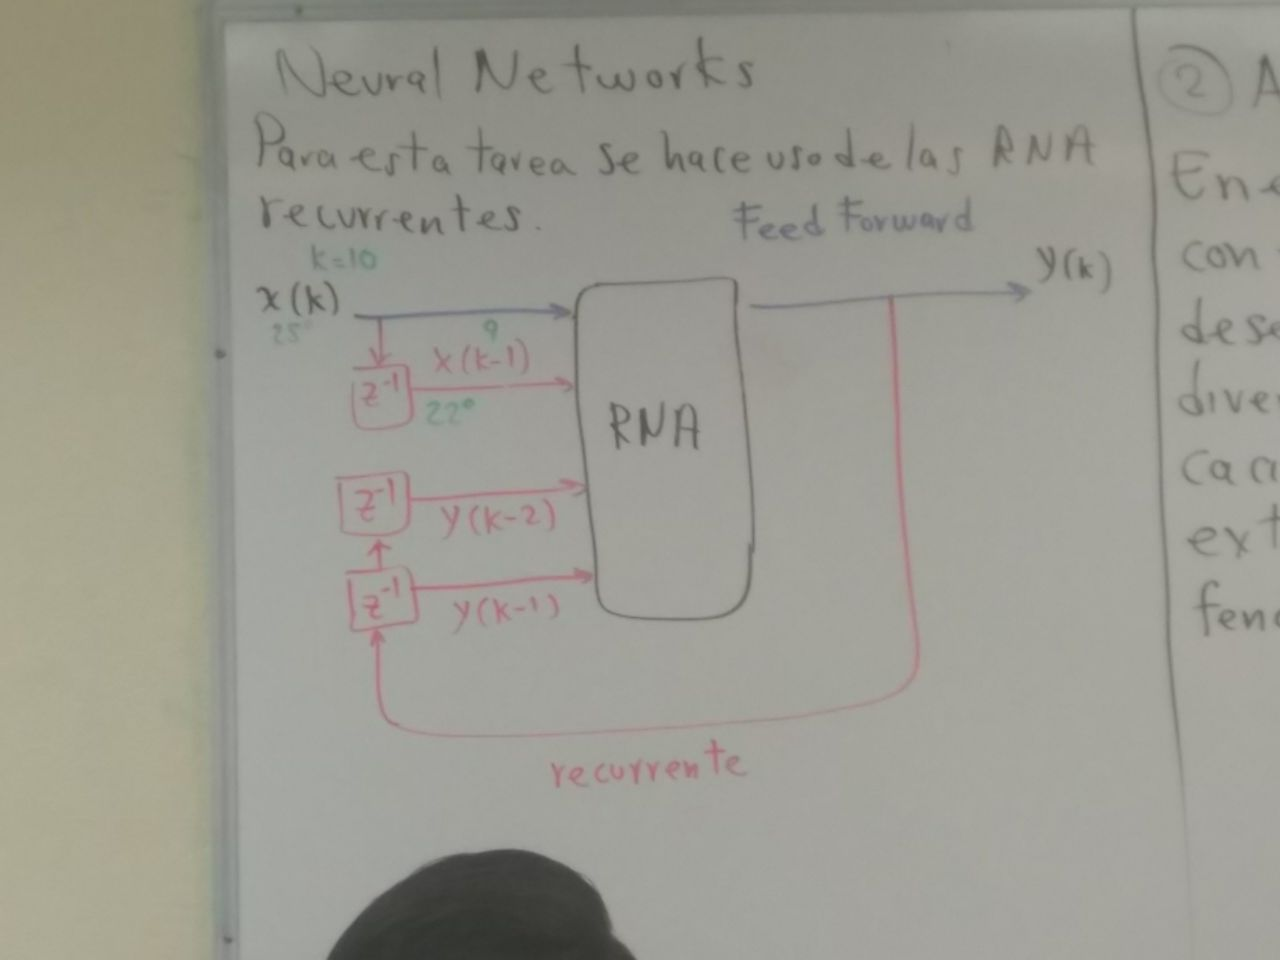
\includegraphics[scale=.37]{recurrentExample2}	
\end{figure}

\section{Control de Sistemas}
Dado un sistema $f(t)$ se requiere modificar su comportamiento para que sea estable. En esta aplicación se usa una RNA para aproximar a $f(t)$ y una RNA para diseñar un controlador.

\begin{figure}
	\centering
	\caption{System Control Example}
	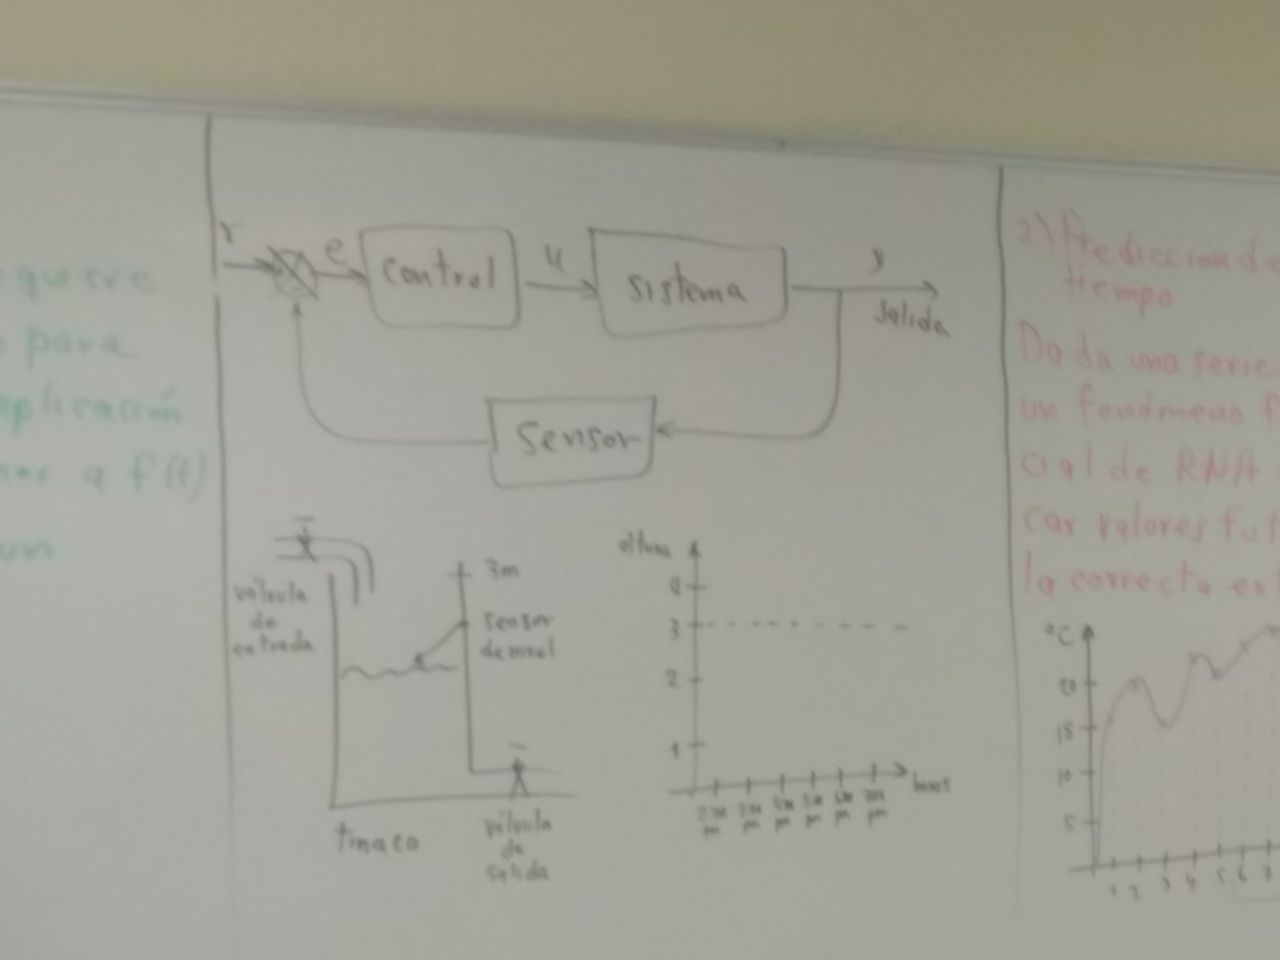
\includegraphics[scale=.37]{systemControlExample1}	
\end{figure}

\part{Aplicaciones de la RNA}
\section{Reporte de Práctica}
\begin{enumerate}
	\item Intro
	\item Metodología
	\item Pseudo código
	\item Resultados(Discusión)
	\item Conclusiones
	\item Referencias(mínimo 2)
\end{enumerate}
\section{Clasificación de Objetos}
Consiste en tener una adecuada separación de un conjunto de objetos mediante una función de semejanza.
\begin{enumerate}
	\item Clasificación supervisada:\\
	Aquí se cuenta con un conjunto de objetos y se conoce a que clase pertenence cada uno de ellos.\\
	Una RNA en modo clasificador puede usar una o más salidas para represtnar a que calse considera que un dato de entrada pertenece.\\
	Aquí tenemos targets ya que tenemos un conjunto de clases a las que este se puede etiquetar.\\
	Las redes pueden ser entrenadad no supervisadamente y supervisadamente\\
	Ejemplos:
	\begin{itemize}
		\item \begin{figure}[h!]
			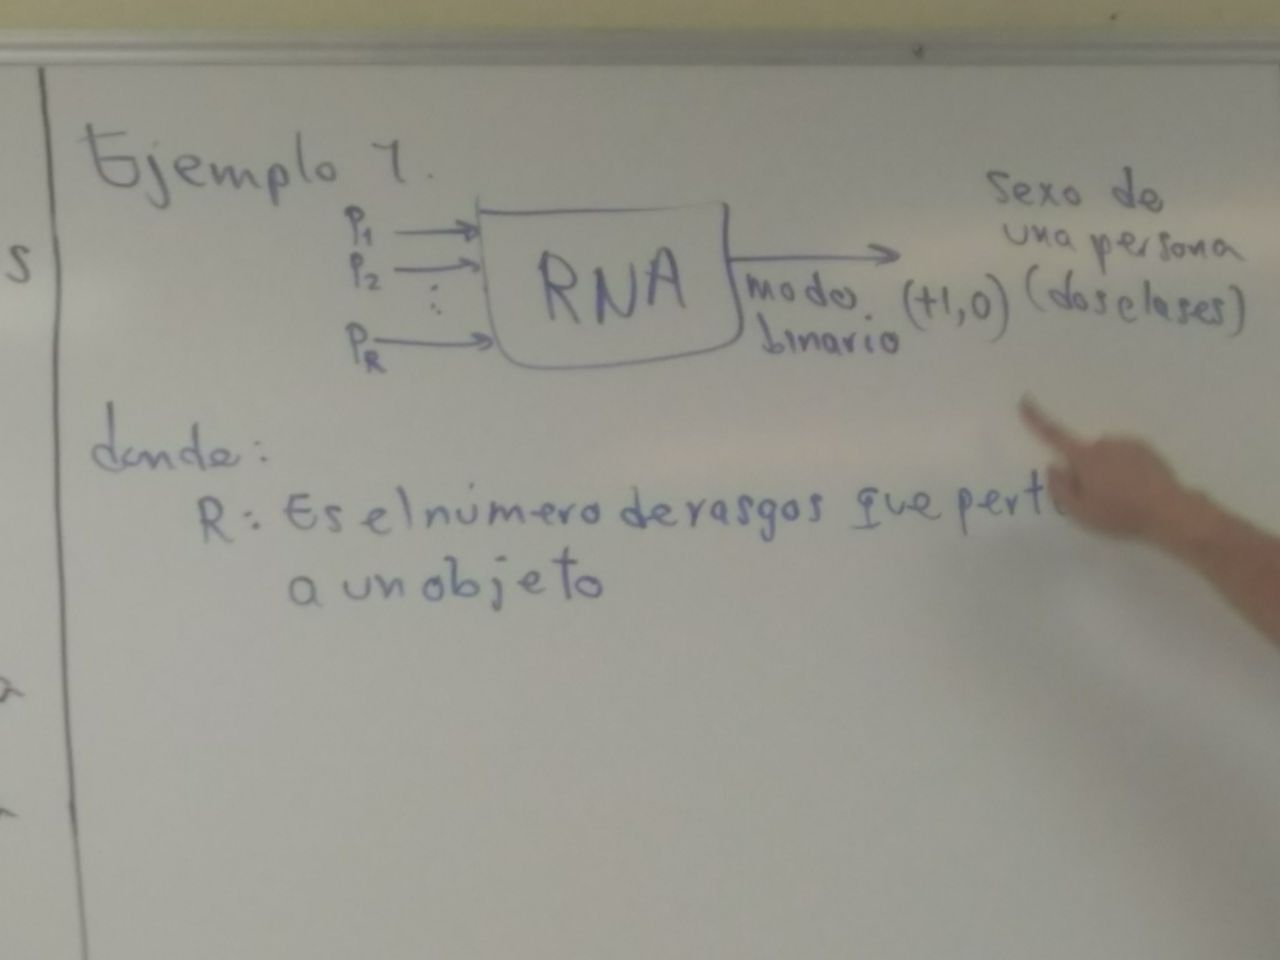
\includegraphics[scale=.2]{appEx1}
		\end{figure}
		\item \begin{figure}[h!]
			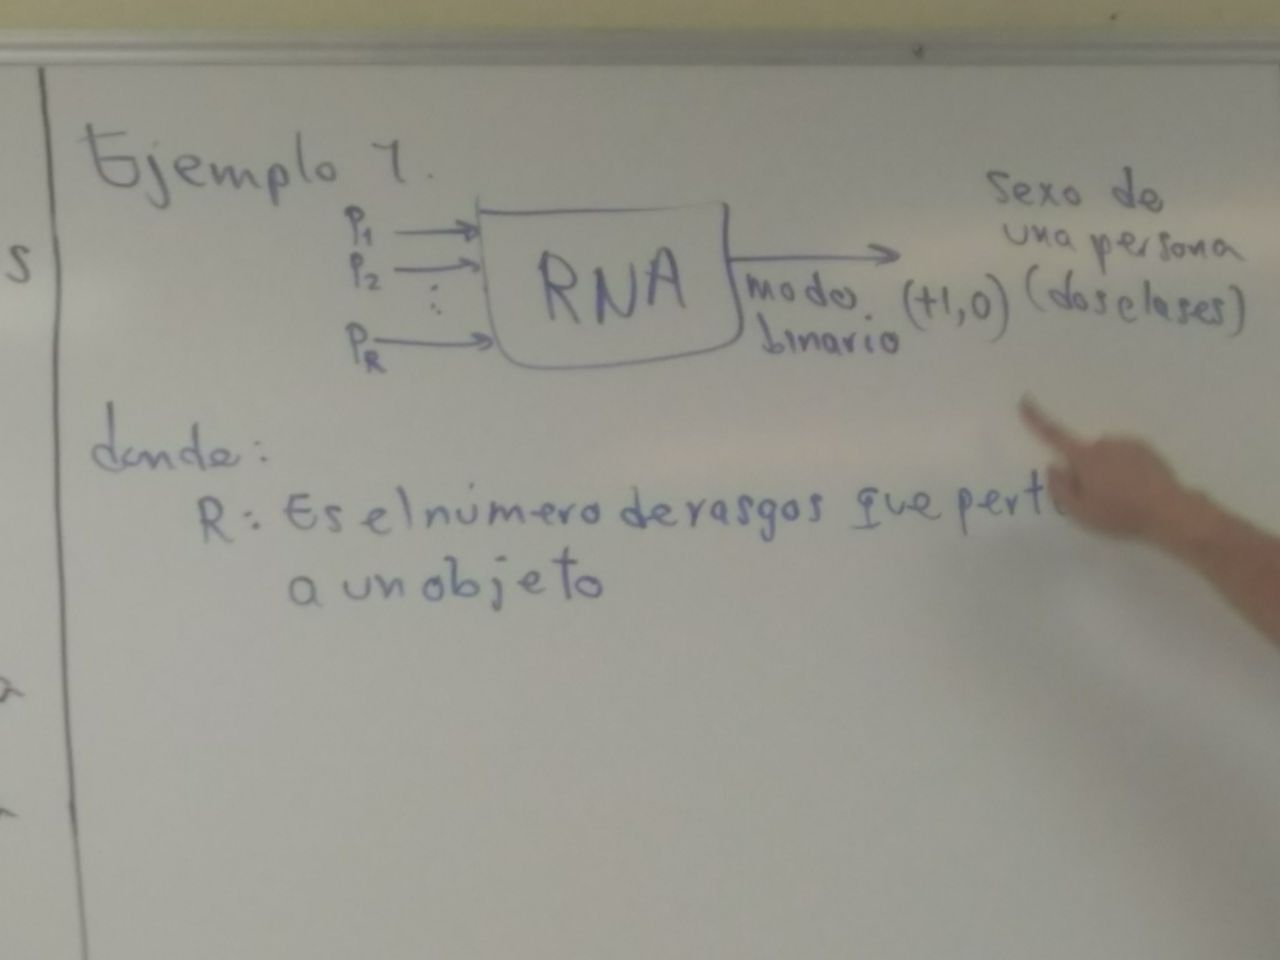
\includegraphics[scale=.2]{appEx2}
		\end{figure}
	\end{itemize}

\end{enumerate}
\section{Neurona Biológica}
Los sistemas biolgcos son tan complejos que se han convertido en una excelente fuente de inspiración para diseñar sistemas artificiales, que emulen algunas de sus características, entre ellas se encuentras las siguientes
\begin{enumerate}
	\item No siempre requieren de módulos de referencia (targets)
	\item Se desempeñan exitosamente ante incertidumbres
	\item Se adaptan fácilmente a nuevos ambientes
	\item Pueden Procesar información de diversas fuentes en forma simultánea
\end{enumerate}
Dado que las RNA nacieron de los elementos básicos de una neurona biológica, es bioinspirada.\\
Los componentes básicos de una neurona biológica son:\\
\begin{figure}[h!]
	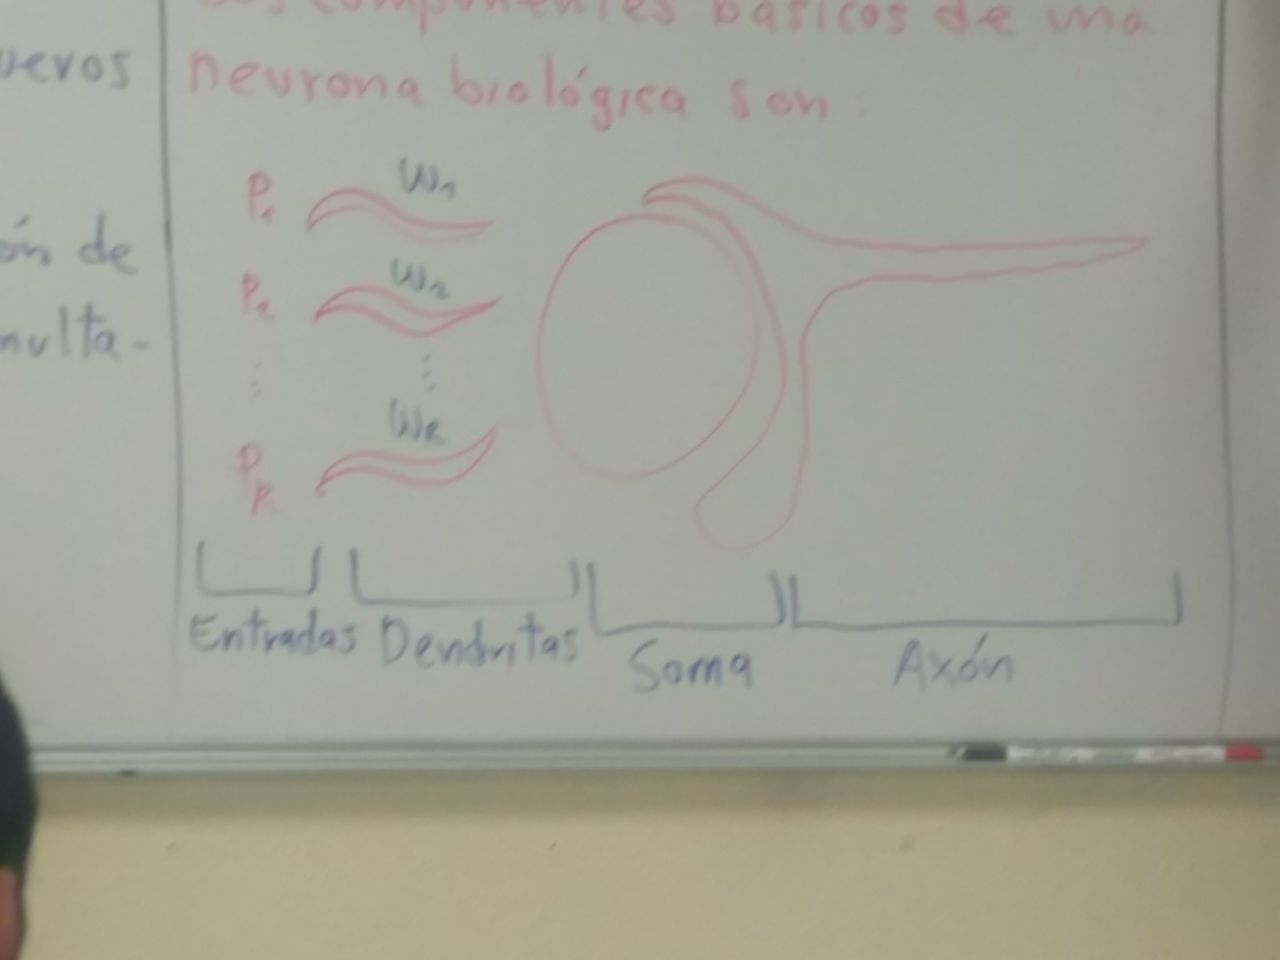
\includegraphics[scale=.20]{bioNeuron}
\end{figure}\\
donde:\\
$P_1,\ldots,P_r$: Son Entradas\\
$W_1, \ldots, W_r$: Son los pesos sinápticos\\
Los pesos sinápticos se usan para indicar el nivel de importancia de cada una de las conexiones para una tarea particular.\\
El soma se encarga de acumular energía y determinar cuando se generará una señal de salida.\\
\textbf{Nota: Para un target o tarea deseada, aprendizaje es buescar un conjutno de $W_1$ a $W_r$ tales que la salida de la red desea igual al target, para todos los datos del conjutno de entramiento}
\end{document}
